\chapter[SM-ID of block structured nonlinear systems]{Set-membership identification of block structured nonlinear systems}

\section{Introduction}
Let us continue to generalize our Set-Membership identification framework introducing the theoretical concepts useful to identify \textbf{SISO nonlinear systems} in the regression form we have seen in the very first part of these notes:

\begin{figure}[h]
   \centering
   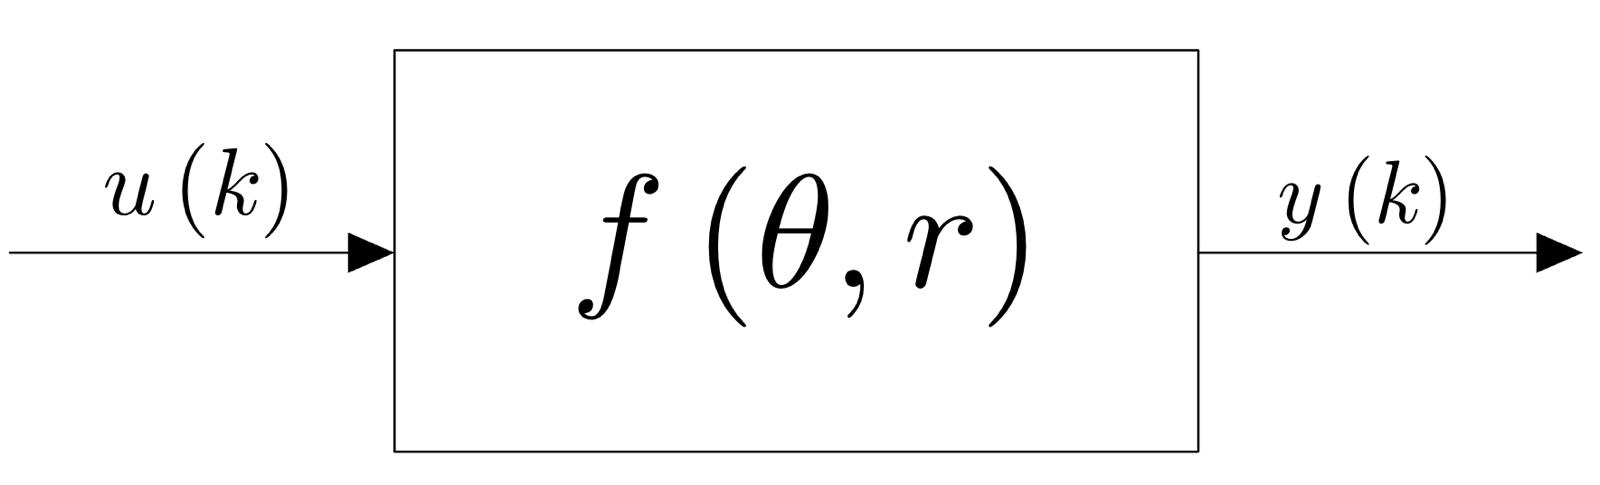
\includegraphics[scale=0.15]{img/nonlinear.jpeg} 
   \caption{Nonlinear SISO system (regression form)}
\end{figure}
\vspace{-1cm}
\begin{equation}
    y(k)=f(\theta,r(k))=f(\theta, [y(k-1),y(k-2),\dots,y(k-n), u(k), u(k-1), \dots, u(k-m)])
\end{equation}
where $\theta$ is the vector with the parameters of the model, while $r(k)$ is the so-called \textbf{regressor}. We specialize the class $f$ of functions we deal with, in particular they are \textbf{multivariate polynomial function of the regressor $r(k)$}. In this context we propose some examples which, as usual, are useful to both introduce and better clarify the setting to which we are approaching. Through all of the examples we do two fundamental quantities are:
\begin{itemize}
    \item The \textbf{dynamical order of the system} $n$; this is related to the number of past samples we need in order to describe the generic system output $y(k)$; 
    \item The \textbf{degree} (or \textbf{order}) $\deg(f)$ of the multivariate polynomial $f$ describing the nonlinear system in the parametrized form.
\end{itemize}

\subsubsection{Example 1}
Suppose that from the physical insights we know that the system has $n=1$ and $\deg(f)=2$. This is the same to state that the equation describing the I/O of the system is:
\begin{align}
    y(k)&=f(\theta,r(k))=f(\theta,[y(k-1),u(k),u(k-1)])=\\
    &=\theta_1y(k-1)+\theta_2 u(k) + \theta_3 u(k-1) 
    + \theta_4 y^2(k-1)+\theta_5 u^2(k)+\theta_6 u^2(k-1)+\\
    &+\theta_7{y(k-1)u(k)}+\theta_8{y(k-1)u(k-1)}+\theta_9{u(k)u(k-1)}
\end{align}

Since $\deg(f)=2$, in order to avoid loosing of generality we have to consider also the mixed monomial terms of order 2.

\subsubsection{Example 2}
Let us consider, now, the case in which both the dynamical order and multivariate polynomial degree are the same as before, on the other hand from the physical insights we know that the structure of the I/O equation is:
\begin{equation*}
    y(k)=\theta_1y(k-1) + \theta_2 u(k) +\theta_3 u^2(k-1)+\theta_4{y(k-1)u(k)}
\end{equation*}
It is not said that all of the terms are present, in this case there is some reason for which this happens.

\subsubsection{Example 3}
Finally, here we consider the case in which, again, $n$, $\deg(f)$ are equal while not having any useful physical insights which can allow us make a guess on the shape of $f(\theta,r)$.
In this particular case some general assumptions on the continuity\footnote{
    for example $f\in\mathcal{C}^0$ or $f\in\mathcal{C}^1$
} of $f$ are needed, otherwise we cannot say anything and the identification problem is not tractable. This example gives the possibility to introduce to cite an important result.

\section{Dealing with nonlinearity of the problem}
Whether one can assume that the function $f$ can leverage on some continuity properties,the \textbf{Stone-Weirstrass theorem} can be used. It allows us with the possibility to approximate as well as we want the true nonlinear function with a multivariate polynomial over a \textit{compact set}. In spite this is a nice result, it is not going to provide a way to build such polynomial, since it is an \textit{existency theorem}.

\subsection{On the choice of the polynomial structure}
When we are not provided with physical insights making us to neglect some terms of the multivariate polynomial, we can always start from a \textit{complete description}, next when the identification procedure is performed, the terms which are not included into the model description will have an uncertainty interval whose central estimate is approximatively equal to zero.

Having said that, the choice of $\deg(f)$ can be done by using the following \textbf{procedure}: 
\begin{enumerate}
    \item[0.] We can start from \footnote{
        If there was $\deg(f)=1$ the system under study is linear
    }$\deg(f)=2$ and we try to solve the problem going through the computation of the feasible parameter set $\mathcal{D}_\theta$ putting together all the available information;\item[1.]\textbf{\large Is the $\mathcal{D}_\theta$ empty?}\footnote{
        Practically speaking, using \texttt{SparsePOP} a symptom of the fact that $\mathcal{D}_\theta=\varnothing \ \iff $ POP infeasible can be read in the output variable \texttt{exitflag}, in particuar its negativeness implies the infeasibility of the POP. 
    }
    \begin{itemize}
        \itemsep-0.3em
        \item {\Large{\color{green}\underline{\textbf{NO}}}} In this case we have to check what are the (relaxed) PUI, in particular we have to check that
        \begin{equation} \label{eq:extrema_sign}
            \text{sign}(\underline{\theta}_i) = 
            \text{sign}(\overline{\theta}_i) \quad i=1,\dots,n_\theta
        \end{equation} 
        Whether this is the case we can accept our solution and use the retrieved interval in order to simulate control the identified system. On the other hand, we continue to investigate in the fact that, maybe the the length of the PUI
        \begin{equation}
            \vert \underline{\theta}_i-\overline{\theta}_i \vert \le \delta
        \end{equation}
         for some small $\delta$. In pratice this is the case when, if for the other parameters the property (\ref{eq:extrema_sign}) is fulfilled, the procedure is saying us that $\theta_i=0$. On the contrary if (\ref{eq:extrema_sign}) is not satisfied and the noise bound is big\footnote{
            We can quantify it in percentage terms with respect to the measured input $\tilde{u}(k)$ or output $\tilde{y}(k)$.
         }, it would be better if the sensor is changed because it is not properly measuring the data to be used in the identification process. Finally on the other side when the \textit{sign concordance property} is not fulfilled and the noise relative bound is acceptable, \textbf{the order of the polynomial ought to be increased} $\to$ try $\deg(f)=\deg(f)+1$. 
     \end{itemize} 
    \item {\Large{\color{red}\underline{\textbf{YES}}}} Also in this case the $\deg(f)$ is too \textbf{low}, then you have to increase it.
\end{enumerate}

\noindent
\begin{remark}[\textbf{Unknown dynamical order} $n$]
    A similar \textit{trial and error} approach can also be applied to the case (both linear and nonlinear systems) when the \textit{dynamical order $n$} is not exactly known from the physical insights. This will be useful especially when the Direct Data-driven control technique will be explained.
\end{remark}

\noindent
\subsection{Additional comments on the PUIs extrema sign concordance}
After this discussion, let us give further attention on the property (\ref{eq:extrema_sign}). The reason why we must reject the PUIs with non-concordant sign is that we cannot even know the sign for a certain parameter. Whether we want to design a simple stabilizing \textit{feedback controller}, the fact that we do not have the information on the sign does not protect us from building a positive feedback(!), making unstable the closed loop system. We conclude this part saying that the \textbf{relative size of the uncertainty} is given by: 
\begin{equation}
    \Delta_i = \bigg\vert \frac{\overline{\theta}_i-\underline{\theta}_i}{\theta_i^c} \bigg\vert, \qquad
    \theta_i^c = \frac{\overline{\theta}_i+\underline{\theta}_i}{2}
\end{equation}
where $\theta_i^c$ is the so-called \textbf{central estimate}  which can leverage on some nice properties how we will see in one of the next chapters. When the sign of the extrema is not the same, the uncertainty relative size is greater than the 1 (that is 100\%).

\section{Toward the computational load reduction}
We have seen in the previous sections a trial and error procedure for choosing either the dynamical order or the order of the multivariate polynomial $f$. The drawback of such an approach is that the computational complexity explode when the such a polynomial have high order. Practical examples are the best way to understand things. Let us do, then, an example.

\subsubsection{Example}
Suppose we want to estimate the parameters of the following nonlinear MISO system:
\begin{equation*}
    y(k)=\theta_1{u_1(k)}+\theta_2{u_1(k)u_2(k)}+\dots+
    +\theta_p{u_1(k)\dots{u_p(k)}}
\end{equation*}
If we add the fact that both the inputs and the output are corrupted by bounded measurement noise. The feasible parameter set is defined as:
\begin{equation}
    \begin{aligned}
        \mathcal{D}_\theta = \{
        \theta\in\mathbb{R}^p: \ &\tilde{y}(k)-\eta(k) = \theta_1 (\tilde{u}(k)-\xi_1(k)) + \theta_2 (\tilde{u}_1(k)-\xi_1(k)) (\tilde{u}(k)-\xi_2(k)) +\dots\\
        &\theta_p (\tilde{u}_1(k)-\xi_1(k))\dots(\tilde{u}_p(k)-\xi_p(k)) \quad k=n+1,...,N\\
        &\vert \eta(k) \vert \le \Delta_\eta \ k=1,...,N\\
        &\vert \xi_i(k) \vert \le \Delta_xi \ k=1,...,N \ i=1,...,p
    \}
    \end{aligned}
\end{equation}
Now, considering the problem of computing the PUIs, we have to solve a POP whose constraints are at most of order $p+1$. Moreover, if $p$ is high, the minimum order of relaxation $\delta_{min}$ is high. Bad symptom! In order to \textbf{reduce the computational complexity} of the POP we can reformulate it by introducing new variables $z_j$ as follows:

\begin{equation*}
    \begin{aligned}
        &\min_{\theta,\xi,\eta,z}  \theta_1\\
        &\text{s.t.} \quad z_1(k)=\xi_1(k)\cdot\xi_2(k), \ 
        z_2(k)=z_1(k)\cdot\xi_3(k), \ \dots, \ z_{p-1}(k)=z_{p-2}(k)\cdot{\xi_p}(k)\\
        &\tilde{y}(k)-\eta(k)=\theta_1{u_1(k)}+\theta_1{\xi_1(k)}+\theta_2+\dots+\theta_p{z_{p-1}}
    \end{aligned}
\end{equation*}
All of the constraints entering the optimization problem are now bilinear, then we can pick as minimum order of relaxation $\delta_{\min}=1$.

\section{Block-oriented nonlinear systems}
The SysId procedure for nonlinear system is quite challenging. When we have addressed the problem of identifying an LTI system (both SISO and MIMO), we had the information about the transfer function that was of crucial importance. For nonlinear system we cannot exploit such an information. In the most general case, assuming we can do some continuity assumptions, we can go through the steps we have described in order to identify the system, otherwise we have to exploit as much as possible the \textit{a-priori information} available on that system. In many situations we can know something about the \textbf{internal structure of the nonlinear system}. To this aim we propose the so-called \textbf{block-structured nonlinear systems}.

\begin{definition}[Block oriented nonlinear systems] Block oriented nonlinear systems are nonlinear dynamical systems which are obtained by \textbf{connecting together} a number of subsystems such that each one of the subsystems can either be:
\begin{itemize}
    \itemsep-0.4em
    \item a \textit{dynamical LTI system}
    \item a \textit{static nonlinear system}
\end{itemize}

\end{definition}

\subsection{Hammerstein system}

This structure is characterized by the following features:
\begin{enumerate}
    \itemsep-0.3em
    \item Internal signal $x(k)$ cannot be measured;
    \item It is useful to describe physical systems which are essentially LTI systems but with a \textbf{significant input nonlinearity} such as input saturation, dead-zone and any other non linear effect in the actuation part.
\end{enumerate}
\begin{figure}[h]
    \centering
    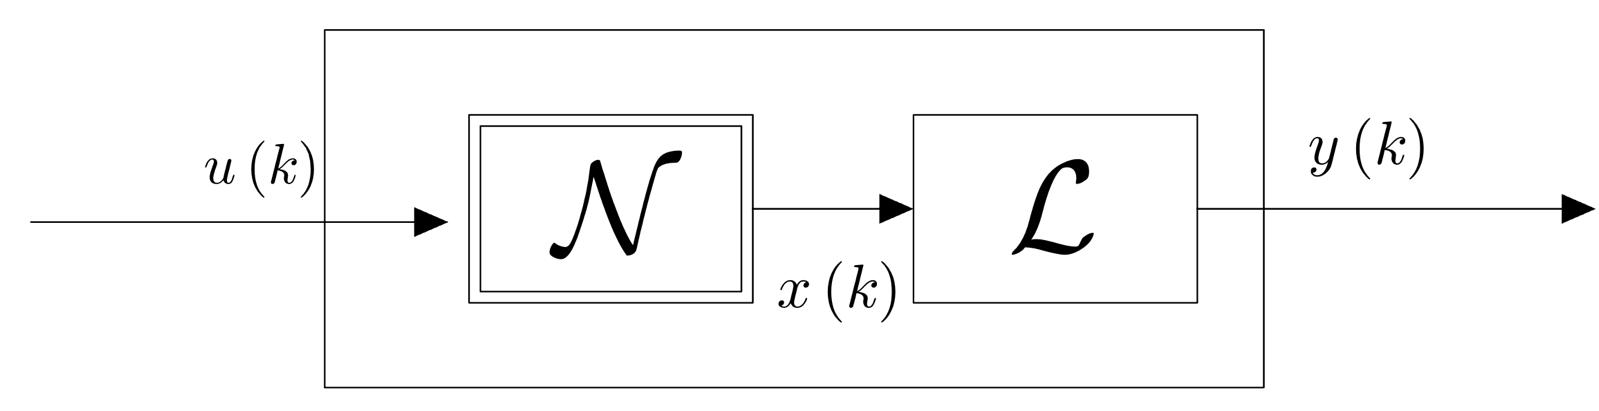
\includegraphics[scale=0.2]{img/hammer.jpeg}
    \caption{Hammerstein system (block diagram)}
\end{figure}

\subsection{Wiener system}
The \textbf{Wiener system} has the nonlinear part $\mathcal{N}$ toward the output. $\mathcal{N}$ is a \textit{linear static map} from the output of the linear system to the output of the nonlinear block.
\begin{figure}[h]
    \centering
    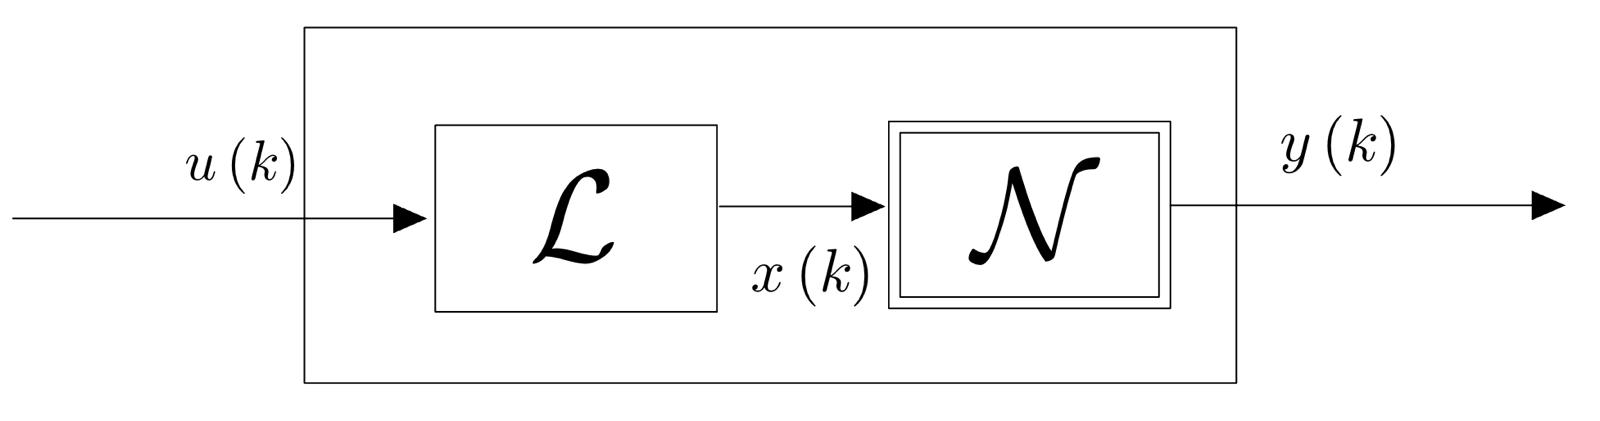
\includegraphics[scale=0.2]{img/Wiener.jpg}
    \caption{Wiener system}
\end{figure}
\begin{remark}[\textbf{Features of the Wiener system}]
    (i) the $x(k)$ signal cannot be measured; (ii) such a type of system is useful to describe systems which are essentially LTI but with a significant \textbf{ouput nonlinearity}.
\end{remark}
When dealing with \textbf{block-structured} systems, we assume that the nonlinear static subsystems can be described by means of polynomial functions, so that all the unmeasurable inner signal will be considered as optimization variables in the SysId problem. 
\section{SM-ID of an Hammerstein system}
\subsection{
    More details on the blocks
}
In the Hammerstein system,the nonlinear part is often referred as $\mathcal{N}(\cdot)$ and it is a function of $u(k)$, while the linear part $\mathcal{L}$ is represented by a transfer function $G(q^{-1})$. Then: 

\begin{equation}\label{eq:hammer}
    \begin{cases}
        y(k)&=-\alpha_1{y(k-2)}-\alpha_2{y(k-2)}-...-\alpha_n{y(k-n)}+\\
        &\beta_0{x(k)}+\beta_1{x(k-1)}+...+\beta_n{x(k-n)}\\
        x(k)&=\mathcal{N}(u(k))
    \end{cases}
\end{equation}
where $\mathcal{N}(\cdot)$ is a \textbf{static linear map} between the input $u(k)$ and the internal output $x(k)$.\\
As an \textit{additional a-priori information} about the structure of the static map, we can saym that:

\begin{equation}
    \begin{aligned}
        x(k)&=\mathcal{N}(u(k))=\sum_{j=1}^m {\gamma_j \ \phi_j\ (u(k)) }=\\
        &=\gamma_1\ {\phi_1\ (u(k))}+\gamma_2 \ {\phi_2\ (u(k))}+...+\gamma_m\ {\phi_m\ (u(k))}
    \end{aligned}
\end{equation}
$\{\phi\}_j$, $j=1,...,m$ is a \textbf{set of basis function} selected on the base of our physical insights. In the case we do not have any other specifical information on the form of $\mathcal{N}$, we can surely selected (keeping in mind the Stone-Weirstrass theorem) the \textit{standard polynomial basis function}:
\begin{equation*}
    \phi_j=u^j(k) \quad   \forall j=1,...,m
\end{equation*}    

\subsection{System Identification procedure}
As usual at this stage, when we want to formulate the problem of SysId we havo to put together a-priori and a-posteriori information. \begin{description}
    \item[\textbf{Prior information on the system}] Since we have said that the system is an \textit{Hammerstein one} we know that:
    \begin{enumerate}
        \item \textsc{Nonlinear part ($\mathcal{N}$)} can be espressed how we have just seen. Moreover, note that there is no constant term (in other words there is no term with the power 0), since it is of little practical interest.
        \item \textsc{Linear part ($\mathcal{L}$)} is described by $y(k)$ as in equation (\ref{eq:hammer})
    \end{enumerate}
    \item[\textbf{Prior information on the noise}] Here we assume an \textbf{Output Error (OE)} setting for sake of simplicity. We assume as always the boundedness of the noise samples
    \begin{equation*}
        \vert \eta(k) \vert \le \Delta_\eta \quad k=1,...,N
    \end{equation*}
    \item[\textbf{A-posteriori information: collected data}] Are the $N$ pairs $(u(k),\tilde{y}(k))$ experimentally collected by performing an open-loop experiment on the plant.
\end{description}

\noindent
Putting all together we can retrieve the    \textbf{Feasible parameter Set} where the parameters are $\theta=[\alpha_1 \dots \alpha_n \ \beta_0 \dots \beta_n \ \gamma_1 \dots \gamma_m]$\footnote{
    We can also split them into two parts: $\gamma$ that are the ones related to $\mathcal{N}$ and $\theta$ which are the ones related to $\mathcal{L}$.
}: 
\begin{equation}
    \begin{aligned}
        \mathcal{D}_\theta=\big\{
        \theta\in\mathbb{R}^{2n+1+m}: \ 
        &y(k)=-\alpha_1{y(k-1)+...+\beta_n{x(k-n)}} \quad \forall{k=n+1,...,n}\\
        & x(k)=\gamma_1{u(k)}+\gamma_2{u^2(k)}+...+\gamma_m{u^{m}(k)} \ k=1,...,n \\
        &\tilde{y}(k)=y(k)+\eta(k), \quad 
        \vert \eta(k) \vert \le \Delta_\eta \quad k=1,..., N
    \big\}
    \end{aligned}
\end{equation}

\noindent
We know that we have to go on by computing the minimum for each theta in the derived set, that must be extended. There are mainly two approaches by which we can go on. In the former we \textit{eliminate the dependence on the inner variable $x$} by substituting it in the expression defining $\mathcal{L}$ while the former is about considering also the samples of the inner signal $x(k)$ as optimization variables. In the following we will consider separately the parameters of the static and the dynamic block of the overall Hammerstein system.

\begin{figure}
    \centering
    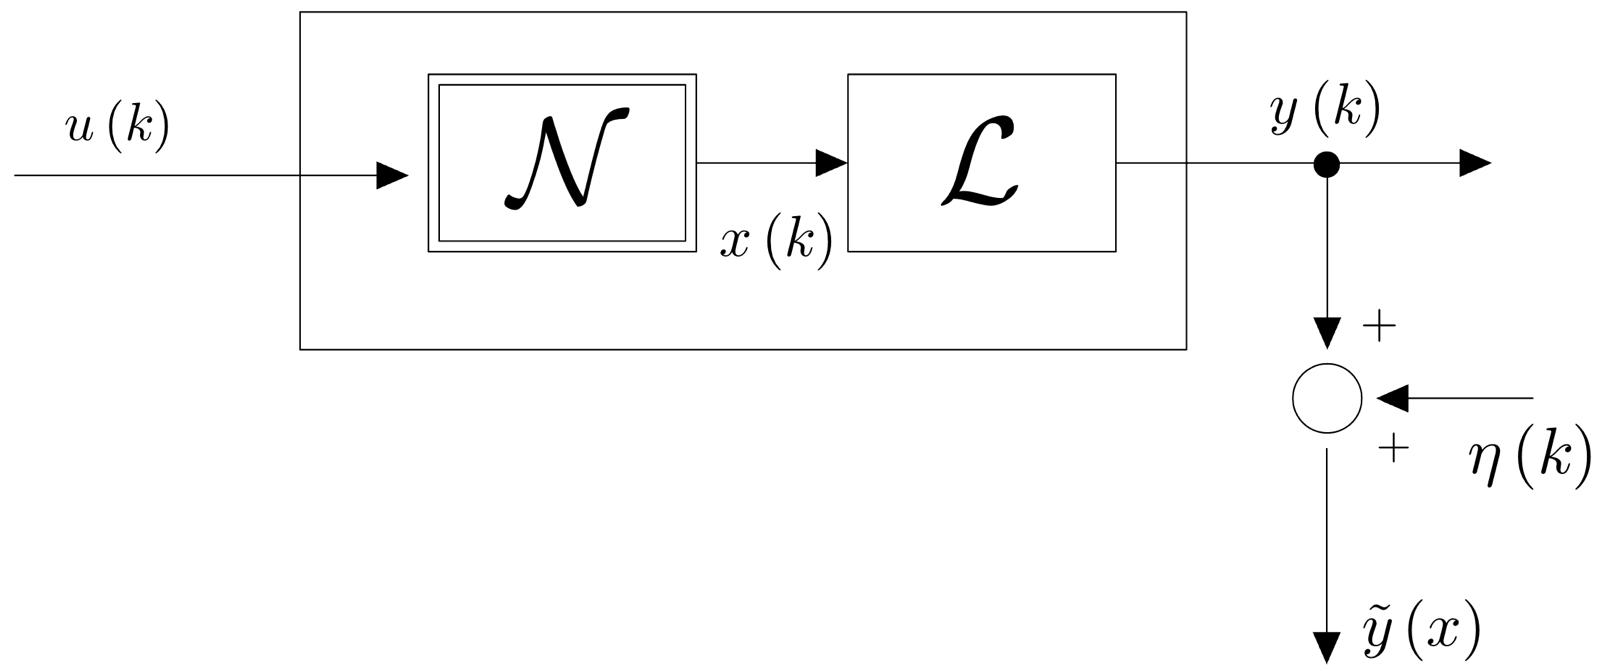
\includegraphics[scale=0.2]{img/hammer_OE.jpg}
    \caption{Hammerstein system (OE setting)}
\end{figure}

\subsection{First approach: toward the definition of $\mathcal{D}_{\theta,\gamma,\eta}$}
By using this first approach, we can eliminate the dependence of the set on $x(k)$ by substituting it in the first equation. The resulting \textbf{Extended feasible parameter set} is:
\begin{equation}
    \begin{aligned}
        \mathcal{D}_{\theta,\gamma, \eta}=\{&
        \theta\in\mathbb{R}^{2n+1}, \gamma\in\mathbb{R}^{m}, \eta\in\mathbb{R}^N: \  
        \tilde{y}(k)-\eta(k)=-\alpha_1[\tilde{y}(k-1)-\eta(k-1)]-\dots-\\
        &-\alpha_n[\tilde{y}(k-n)-\eta(k-n)] +
        \beta_0\gamma_1{u(k)} + \beta_0{\gamma_2}{u^2(k)} +\dots+\beta_0\gamma_m{u^m(k)}+\\
        &+...+\beta_n{\gamma_1}{u(k-n)}+...+\beta_n{\gamma_m}{u^m(k-n)} \quad k=n+1,...,N\\
        &\vert \eta(k) \vert \le \Delta_\eta \quad k=1,...,N
    \}
    \end{aligned}
\end{equation}
This set is defined by bilinear constraints; the PUIs can be computed as usual as: 
\begin{equation}
    PUI_{\theta_j} = [
        \underline{\theta}_j,
        \overline{\theta}_j
    ] \qquad 
    \underline{\theta}_j=\min_{\theta,\gamma,\eta\in{\mathcal{D}_{\theta,\gamma,\eta}}} \ {\theta_j}, \quad
    \overline{\theta}_j=\max_{\theta,\gamma,\eta\in{\mathcal{D}_{\theta,\gamma,\eta}}} \ {\theta_j} 
\end{equation}

\begin{remark}
    \textbf{Approach 1} leads to POPs with:
    \begin{enumerate}
        \itemsep-0.2em
        \item $2n+1+m+N$ variables; 
        \item max degree of the constraints equal to 2; 
        \item N-n \textit{bilinear} polynomial constraints of order 2; 
        \item 2N linear constraints (\small{$\vert \eta(k) \vert \le \Delta_\eta$})
    \end{enumerate}
\end{remark}

\subsection{Second approach: toward the definition of $\mathcal{D}_{\theta,\gamma,x,\eta}$}
Here we are not going to replace the $x(k)$ samples, we consider them as optimization variables. This leads to the following description of the EFPS:
\begin{equation}
    \begin{aligned}
        \mathcal{D}_{\theta,\gamma,x,\eta} = \big\{&
            \theta\in\mathbb{R}^{2n+1}, \gamma\in\mathbb{R}^m, x\in\mathbb{R}^N, \eta\in\mathbb{R}^N:\\
            &y(k)=-\alpha_1{y(k-1)+...+\beta_n{x(k-n)}} \quad \forall{k=n+1,...,n}\\
            & x(k)=\gamma_1{u(k)}+\gamma_2{u^2(k)}+...+\gamma_m{u^{m}(k)} \ k=1,...,n \\
            &\tilde{y}(k)=y(k)+\eta(k), \quad 
            \vert \eta(k) \vert \le \Delta_\eta \quad k=1,..., N
        \big\}
    \end{aligned}
\end{equation}
Again, we have bilinear constraints and the problem of finding the \textit{parameter uncertainty interval} can be formulated as usual: 
\begin{equation}
    PUI_{\theta_j} = [
        \underline{\theta}_j,
        \overline{\theta}_j
    ] \qquad  
    \underline{\theta}_j=\min_{\theta,\gamma,x,\eta\in{\mathcal{D}_{\theta,\gamma,x,\eta}}} \ {\theta_j}, \quad
    \overline{\theta}_j=\max_{\theta,\gamma,x,\eta\in{\mathcal{D}_{\theta,\gamma,x,\eta}}} \ {\theta_j} 
\end{equation}

\begin{remark}
    \textbf{Approach 2} leads to POPs with:
    \begin{enumerate}
        \itemsep-0.3em
        \item $2n+1+m+2N$ optimization variables
        \item max degree of the polynomial constraints equal to 2
        \item $N-n$ polynomial constraints of order 2
        \item $2N$ linear constraints (deriving from $\eta,x$)
    \end{enumerate}
\end{remark}

The problem we have just presented satisfy the \textit{running intersection property} so that the \textit{Sparse convex relaxation} can be applied. Moreover the fact that we have bilinear constraints allows us to pick as minimum order of relaxation $\delta_{min}=1$. \\
At this point it seems that all clear and suitable to solve the problem by using \texttt{sparsePOP} (for example). There is another problem to face related to the \textbf{well-posedness} of such a problem.

\section{Identifiability for Hammerstein system}
Let us consider the following Hammerstein systems:
\begin{figure}[h]
    \centering
    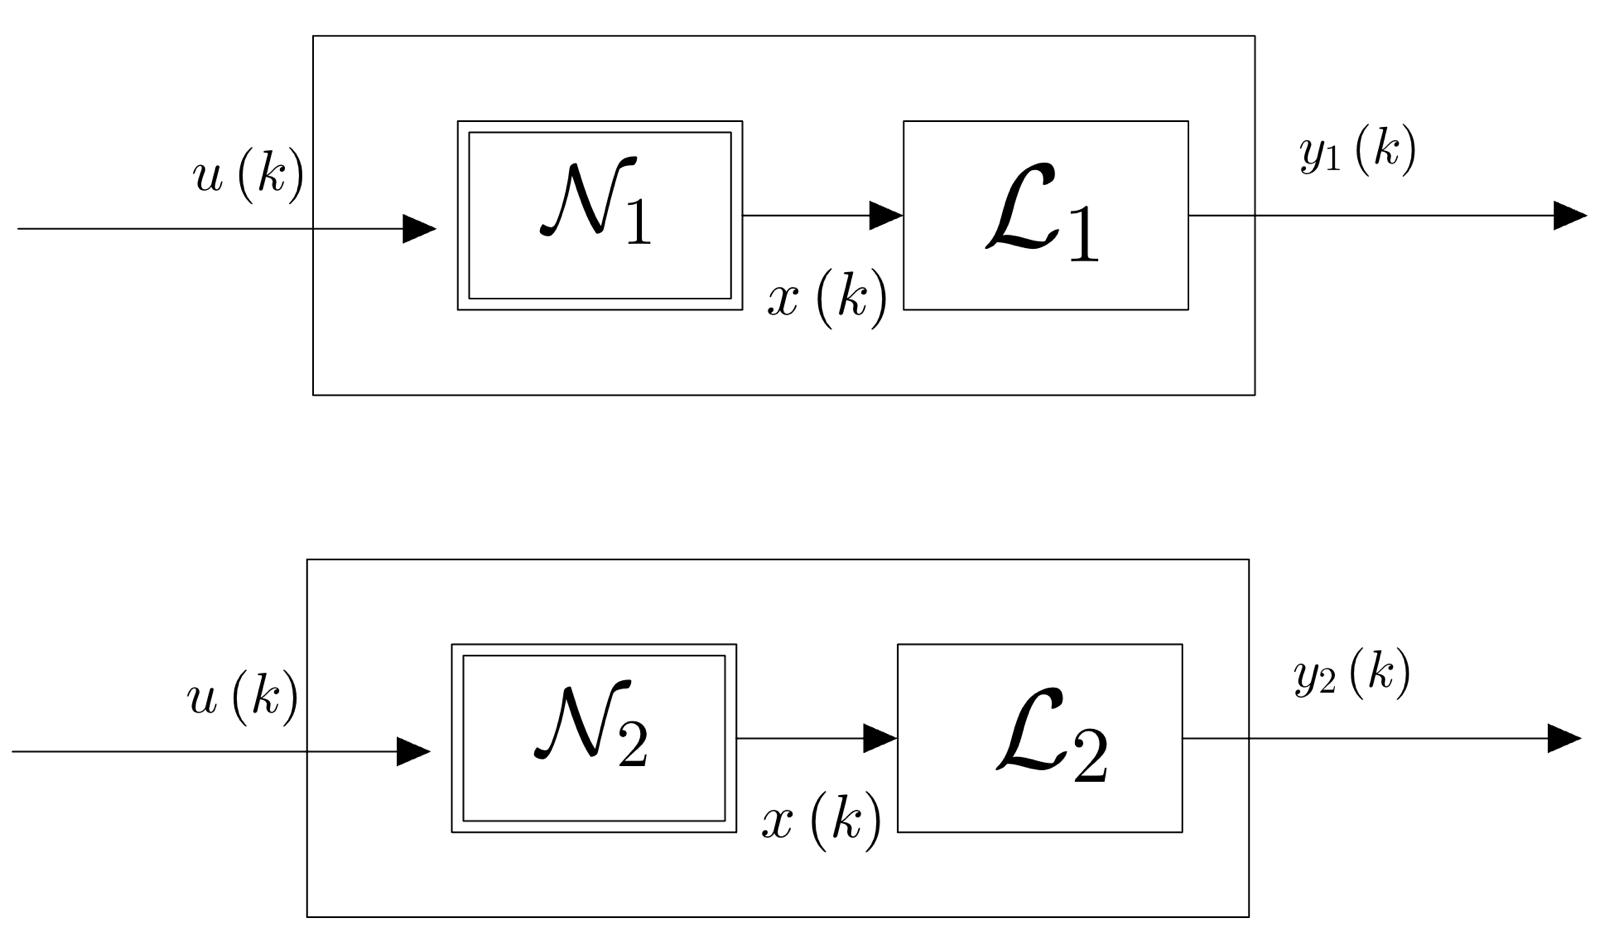
\includegraphics[scale=0.2]{img/twohammer.jpg}
    \caption{Two Hammerstein systems identical from the Input/Output point of view}
\end{figure}

%figure here
\noindent
It can be easily proved that $y_1(k)=y_2(k)$ provided that $\mathcal{N}_2=\mathcal{N}_1/\alpha$ and $\mathcal{L}_2=\alpha\mathcal{L}_{1}$ $\forall\alpha \in \mathbb{R}$. The Hammerstein system is not identifiable because we have an infinite number of solutions of the identification problem which are perfectly equivalent from the input/output point of view. We are able to draw two important conclusions:
\begin{description}
    \item[\textbf{Result 1}] No matter what is the technique that we are going to use we will not be able to estimate the exact parameters of the Hammerstein system generating the data, even if we are collecting \textit{noiseless data} and $N\to\infty$. This leads to an intrinsic \textbf{unidentifiability}.
    \item[\textbf{Result 2}] Since we have an infinite number of \textit{Hammerstein model} which are able to provide exactly the same I/O behaviour of the true one, our numerical procedure for the computation of the PUI \textbf{is going to fail}. This is due to the fact the FPS will be \textbf{structurally unbounded}.
\end{description}

From such results we understand that we need an \textbf{additional constraint}, in principle any constraint so that the I/O behaviour is not changed. For example: 
\begin{enumerate}
    \itemsep-0.2em
    \item We can fix the DC-gain of $G(q^{-1})$ to a given value;
    \item We can fix one of the parameter of $\mathcal{N}$ to a fixed.
\end{enumerate}
In general: any normalization of either G or N is fine! The easiest approach that is not leading to any loss of generality is to set the DC-gain of $G(q^{-1})$ to 1. If we impose such a condition we will obtain another constraint:
\begin{equation}
    \frac{\beta_0+\beta_1+\beta_2+...+\beta_n}{1+\alpha_1+\alpha_2+...+\alpha_n}=1
\end{equation}
This is nothing but a \textbf{linear additional constraint} on the system parameters. 

\section{Extension for non-polynomial $\{\phi\}_j$ basis function}
At this stage we wonder if the presented SM-ID method for the Hammerstein system can be extended to the case where $\mathcal{N}$ is no more polynomial. The answer is positive provided that $\mathcal{N}$ is polynomially parametrized that is: 
\begin{equation}
    \mathcal{N}(\cdot): \ x(k)=\gamma_1{\varphi_1(u(k))}+\gamma_2{\varphi_2(u(k))}+...+\gamma_m{\varphi_m(u(k))}
\end{equation}
This is quite useful when either the nonlinearity is \textbf{difficult} to be approximated by polynomials (hard nonlinearity such as \textbf{input saturation}), or the application explicitly suggests a precise choice of $\varphi_1, \ ... \ , \varphi_m$. This last case arises when we have for example a \textbf{dead zone}.
The following figure from \cite{pupeikis2003identification}: 
\begin{figure}[h]
    \centering
    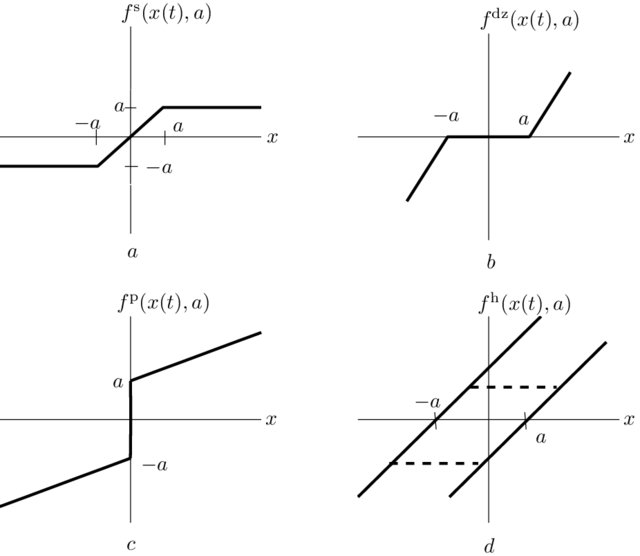
\includegraphics[scale=1.2]{img/hardNL.jpg}
    \caption{Examples of hard nonlinearities}
\end{figure} 

\section{Generalization of SysId of block-structured nonlinear systems using \textit{Linear Fractional Transformation (??)}}
